
\documentclass{standalone}
\usepackage{tikz}
\usepackage{adjustbox}
\usepackage{helvet}  
\usepackage{sansmathfonts}  
\renewcommand{\familydefault}{\sfdefault}  
\usetikzlibrary{arrows.meta,calc,decorations.pathmorphing}
\usetikzlibrary{shapes.arrows}
\usepackage{xcolor}
\definecolor{colorff6633}{HTML}{ff6633}
\begin{document}
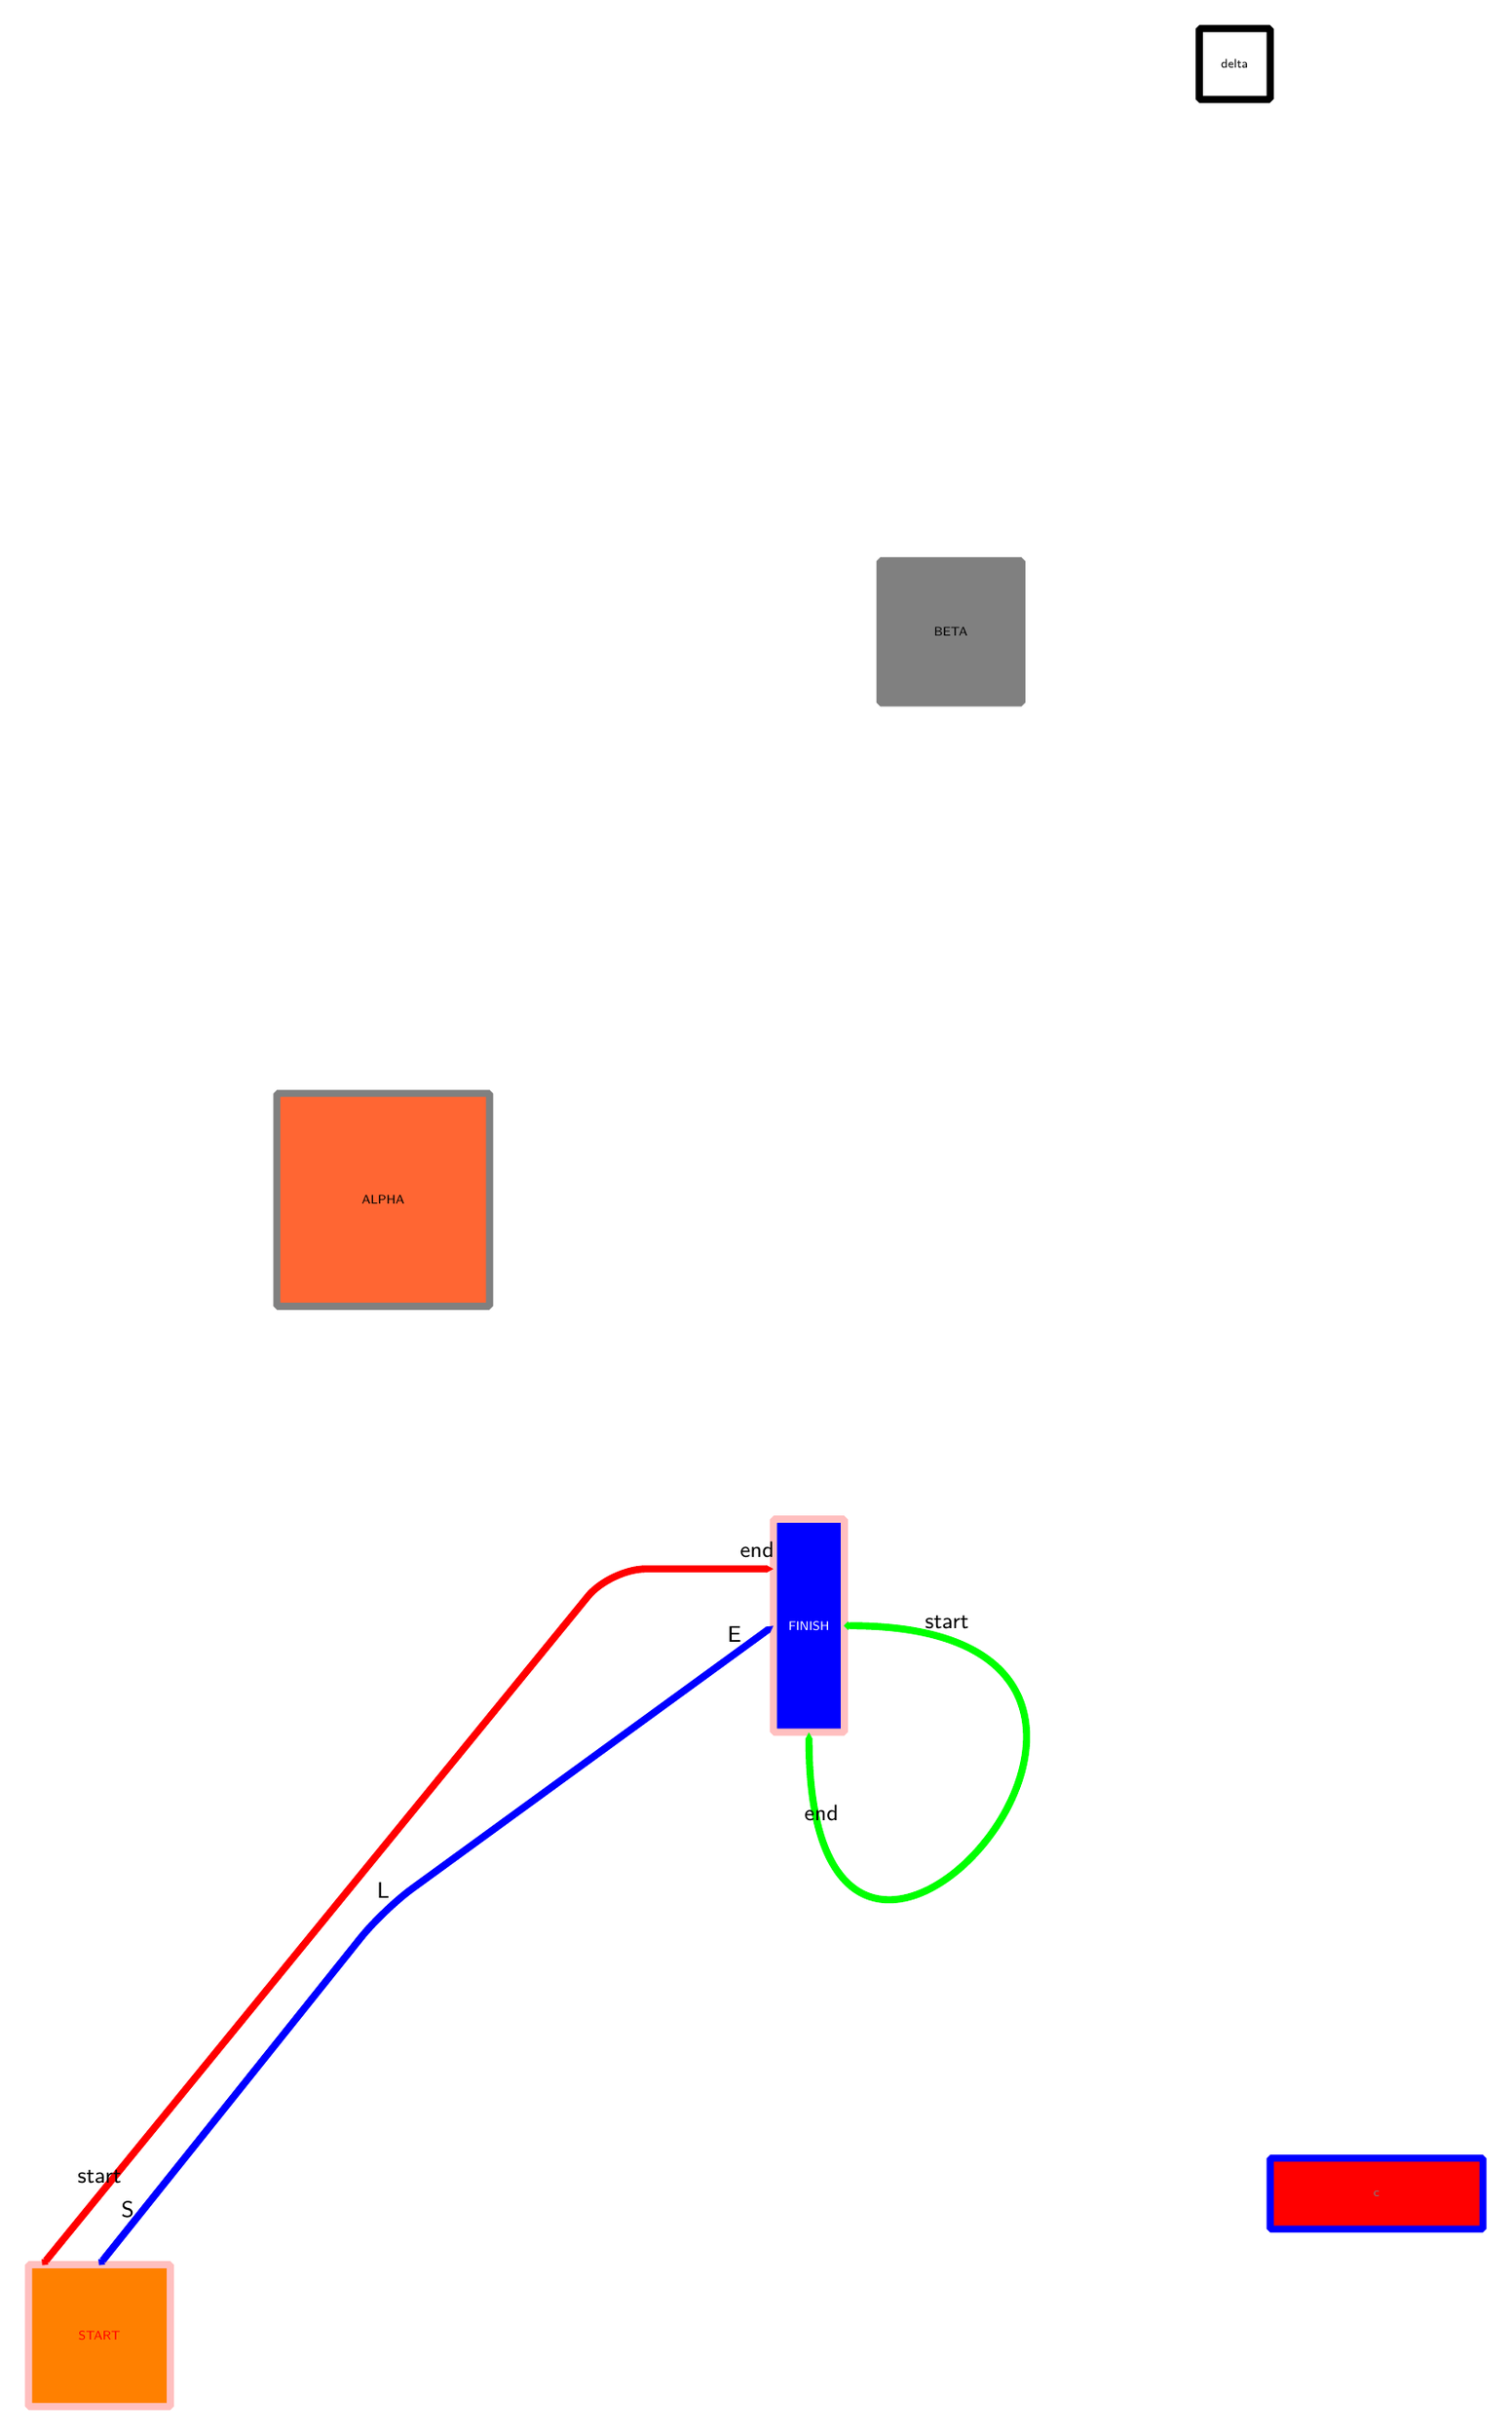
\begin{tikzpicture}
    [>={Stealth[scale=1.0]},  % Uniform arrow style
    ]
    
\node[shape=rectangle, fill=orange, draw=pink, minimum width=2cm, minimum height=2cm, rounded corners=0.025cm, line width=0.1cm, text opacity=1, font=\tiny, inner sep=0pt] (node_a) at (4,4) {\adjustbox{max width=2cm, max height=2cm}{\textcolor{red}{START}}};
\node[shape=rectangle, fill=blue, draw=pink, minimum width=1cm, minimum height=3cm, rounded corners=0.025cm, line width=0.1cm, text opacity=1, font=\tiny, inner sep=0pt] (node_b) at (14,14) {\adjustbox{max width=1cm, max height=3cm}{\textcolor{white}{FINISH}}};
\node[shape=rectangle, fill=red, draw=blue, minimum width=3cm, minimum height=1cm, rounded corners=0.025cm, line width=0.1cm, text opacity=1, font=\tiny, inner sep=0pt] (node_c) at (22,6) {\adjustbox{max width=3cm, max height=1cm}{\textcolor{gray}{c}}};
\node[shape=rectangle, fill=colorff6633, draw=gray, minimum width=3cm, minimum height=3cm, rounded corners=0.025cm, line width=0.1cm, text opacity=1, font=\tiny, inner sep=0pt] (node_alpha) at (8,20) {\adjustbox{max width=3cm, max height=3cm}{ALPHA}};
\node[shape=rectangle, fill=gray, draw=gray, minimum width=2cm, minimum height=2cm, rounded corners=0.025cm, line width=0.1cm, text opacity=1, font=\tiny, inner sep=0pt] (node_beta) at (16,28) {\adjustbox{max width=2cm, max height=2cm}{BETA}};
\node[shape=rectangle, fill=white, draw=black, minimum width=1cm, minimum height=1cm, rounded corners=0.025cm, line width=0.1cm, text opacity=1, font=\tiny, inner sep=0pt] (node_delta) at (20,36) {\adjustbox{max width=1cm, max height=1cm}{delta}};
\draw[draw=green,line width=0.1cm,rounded corners=0.5cm,arrows={Circle[width=0.1cm,length=0.1cm]}-{Triangle[width=0.1cm,length=0.1cm]}] (14.5,14) .. controls (20.5,14) and (14,6.5) .. (14,12.5) node[above, pos=0.1] {\small{\sffamily{start}}} node[above, pos=0.9] {\small{\sffamily{end}}};
\draw[draw=blue,line width=0.1cm,rounded corners=0.5cm,arrows={Circle[width=0.1cm,length=0.1cm]}-{Triangle[width=0.1cm,length=0.1cm]}] (4,5) -- (8,10) node[above, pos=0.1] {\small{\sffamily{S}}} -- (13.5,14) node[above, pos=0.9] {\small{\sffamily{E}}} node[above, pos=0] {\small{\sffamily{L}}};
\draw[draw=red,line width=0.1cm,rounded corners=0.5cm,arrows={Circle[width=0.1cm,length=0.1cm]}-{Triangle[width=0.1cm,length=0.1cm]}] (3.2,5) -- (11.2,14.8) node[above, pos=0.1] {\small{\sffamily{start}}} -- (13.5,14.8) node[above, pos=0.9] {\small{\sffamily{end}}};

\end{tikzpicture}
\end{document}
